% ============================================================
% An Empirical Anatomy of Failure in Small-Model
% Long-Term Conversational Memory
%
% Self-contained: compiles on Overleaf with pdflatex + bibtex,
% no external style files. To submit to a specific venue, replace
% \documentclass and the title block with that venue's style
% (e.g. acl.sty / neurips_2026.sty) -- the \input sections are reusable.
%
% HONESTY POLICY: every number in this paper is a real measured value
% from the accompanying code (github.com/saisushaman/AI-MEMORY-,
% experiments/*.py). No result is fabricated. [PLACEHOLDER] marks any
% value not yet measured; there should be none in the main results.
% ============================================================
\documentclass[11pt]{article}

\usepackage[margin=1in]{geometry}
\usepackage{times}
\usepackage{booktabs}
\usepackage{graphicx}
\usepackage{amsmath}
\usepackage{amssymb}
\usepackage{url}
\usepackage[hidelinks]{hyperref}
\usepackage{xcolor}
\usepackage{authblk}

\newcommand{\mdr}{\textsc{MDR}}
\newcommand{\rtf}{\textsc{RTF}}

\title{\bf An Empirical Anatomy of Failure in Small-Model\\ Long-Term Conversational Memory:\\ Redundancy, Retrieval, and Reasoning}

\author{Sai Sushama}
\affil{\normalsize (author affiliation)}
\date{}

\begin{document}
\maketitle

\begin{abstract}
Long-term memory for large language model (LLM) agents is usually studied one
mechanism at a time---deduplication, retrieval, or consolidation---and almost
always with large frontier models. We instead present a controlled empirical
\emph{anatomy} of where a small, fully local agent-memory pipeline
(\texttt{qwen3:8b} extraction and answering, \texttt{nomic-embed} retrieval)
loses accuracy on the LoCoMo long-term conversational-memory benchmark, judged
by an LLM rater. Three findings emerge. \textbf{(1) Redundancy is real but
semantic, not lexical:} an LLM-built memory store contains up to $62\%$
near-duplicate facts at a cosine threshold of $0.85$, essentially invisible to
exact/lexical matching ($\approx\!0\%$). \textbf{(2) Deduplication does not
help and often hurts:} blindly merging near-duplicates is Pareto-dominated at
every retrieval budget (e.g.\ $0.15$ vs.\ $0.37$ judged accuracy on multi-hop),
and redundancy-aware composition (maximal marginal relevance) is
\emph{statistically indistinguishable} from plain top-$k$ retrieval on multi-hop
questions ($n{=}282$, McNemar $p{=}0.90$ at $k{=}8$). \textbf{(3) The dominant
error source is retrieval precision and reasoning, not redundancy:} with the
benchmark's \emph{gold evidence} in context, accuracy jumps from $0.40$
(retrieval) to $0.61$ (oracle), yet temporal questions remain near-floor
($0.156$) \emph{even with perfect evidence}, and supplying the entire
conversation \emph{underperforms} precise evidence on multi-hop
($0.628$ vs.\ $0.721$). We also observe that grounded extractive memory is
largely faithful ($0/120$ sampled facts unsupported), unlike open-ended
generation. Our contribution is not a new method---the space is
saturated---but a reproducible, honest decomposition that reorders where effort
should go: away from deduplication, toward precision retrieval and, above all,
reasoning/grounding that no amount of retrieval can supply. Code and data:
\url{https://github.com/saisushaman/AI-MEMORY-}.

\end{abstract}

\section{Introduction}

LLM agents increasingly maintain a persistent memory: salient facts are
extracted from conversations, stored, and later retrieved to answer questions
that span many sessions~\cite{packer2023memgpt,chhikara2025mem0,xu2025amem}.
Progress is typically reported one mechanism at a time---better
consolidation, deduplication, graph structure, or retrieval---and almost
exclusively with large frontier models on benchmarks such as
LoCoMo~\cite{maharana2024locomo} and LongMemEval~\cite{wu2024longmemeval}.

This leaves a practical question unanswered: for a \emph{small, locally
runnable} agent-memory stack, \emph{where does the accuracy actually go}? Which
of the many proposed levers---removing redundant memories, retrieving more
precisely, or reasoning better over what is retrieved---would move the needle,
and which are dead ends? Answering this requires holding the pipeline fixed and
decomposing its error, rather than proposing yet another mechanism.

We do exactly that. Using a single small open model (\texttt{qwen3:8b}) for both
extraction and answering, a local embedding model (\texttt{nomic-embed}) for
retrieval, and an LLM judge for scoring, we run a controlled study on LoCoMo and
measure the effect of (i) redundancy in the store, (ii) deduplication and
redundancy-aware composition, and (iii) retrieval precision versus reasoning,
using the benchmark's gold evidence as an oracle ceiling.

\paragraph{Contributions.} We make no methodological claim; recent work already
covers deduplication~\cite{abbas2023semdedup,peng2025adagres}, precision
retrieval over conversational memory~\cite{li2026evimem,ji2026mragent}, and
memory hallucination~\cite{chen2025halumem}. Our contribution is an honest,
reproducible \emph{diagnosis}:
\begin{enumerate}
  \item A redundancy measurement (\mdr/\rtf, \S\ref{sec:redundancy}) showing an
  LLM-built store is $\sim\!62\%$ semantically duplicated at $\tau{=}0.85$ yet
  $\approx\!0\%$ lexically---so redundancy is real but requires semantic
  detection.
  \item A negative result (\S\ref{sec:dedup}): blind deduplication is
  Pareto-dominated at every budget, and redundancy-aware composition gives no
  statistically significant gain over top-$k$ on multi-hop ($n{=}282$).
  \item A bottleneck decomposition (\S\ref{sec:bottleneck}): retrieval precision
  leaves $\sim\!21$ accuracy points on the table, but temporal reasoning is a
  hard floor even with gold evidence, and full-context retrieval \emph{distracts}
  on multi-hop.
  \item A faithfulness observation (\S\ref{sec:faithfulness}): grounded
  extractive memory is largely faithful, contrasting open-ended
  generation~\cite{min2023factscore}.
\end{enumerate}
Together these reorder priorities for small-model agent memory: deduplication is
not the lever; precision retrieval helps but is capped; reasoning/grounding is
the ceiling.

\section{Related Work}

\paragraph{Agent memory systems.} MemGPT~\cite{packer2023memgpt} frames memory as
OS-style paging; Mem0~\cite{chhikara2025mem0} extracts and consolidates salient
facts; A-MEM~\cite{xu2025amem} maintains linked structured notes;
Zep~\cite{rasmussen2025zep} uses a temporal knowledge graph; MIRIX~\cite{wang2025mirix}
uses multiple typed memories. These target end-to-end quality; we instead hold a
minimal pipeline fixed and decompose its error.

\paragraph{Deduplication and redundancy.} SemDeDup~\cite{abbas2023semdedup}
removes semantic near-duplicates from \emph{training data};
AdaGReS~\cite{peng2025adagres} performs token-budgeted, redundancy-aware context
selection over RAG chunks with submodular guarantees. We ask whether such
redundancy handling helps an \emph{agent memory} pipeline and find, on our setup,
that it does not.

\paragraph{Precision retrieval and context distraction.} A large body of work
shows that irrelevant or excess context hurts: ``lost in the
middle''~\cite{liu2023lost}, the harm of plausible
distractors~\cite{cuconasu2024power}, sufficiency over
volume~\cite{joren2025sufficient}, and compression to precise
evidence~\cite{xu2024recomp}. Multi-hop retrieval over static corpora is mature (e.g.\ interleaving retrieval
with reasoning~\cite{trivedi2023ircot}, and graph-based associative
retrieval~\cite{gutierrez2024hipporag}). For conversational memory specifically,
EviMem~\cite{li2026evimem} and MRAgent~\cite{ji2026mragent} perform iterative,
evidence-gap-driven or reasoning-in-the-loop multi-hop retrieval. Our oracle
analysis quantifies \emph{how much} precision headroom exists in a small-model
pipeline and, crucially, where it runs out.

\paragraph{Memory faithfulness and hallucination.}
HaluMem~\cite{chen2025halumem} benchmarks operation-level hallucination in agent
memory; atomic-fact checking is mature (e.g.\
FActScore~\cite{min2023factscore}), and hallucinations are known to
snowball~\cite{zhang2023snowball}. We contribute a small observation: grounded
\emph{extractive} memory writes are largely faithful, unlike open-ended
generation, so hallucinated-memory accumulation is a weak effect in this setup.

\paragraph{Evaluation.} We use LoCoMo~\cite{maharana2024locomo} and adopt
LLM-as-judge scoring, consistent with
MemoryAgentBench~\cite{hu2025memoryagentbench} and the difficulty of string-match
metrics on reformulated answers (\S\ref{sec:setup}).

\section{Experimental Setup}
\label{sec:setup}

\paragraph{Data.} We use LoCoMo~\cite{maharana2024locomo}, 10 multi-session
conversations with per-question gold-evidence turn ids and a category label
(1: multi-hop, 2: temporal, 3: open/commonsense, 4: single-hop, 5: adversarial;
we use 1--4 for the accuracy study). Each conversation also ships
per-session extracted \emph{observation} facts, which we use as a
human-grounded reference in \S\ref{sec:redundancy}.

\paragraph{Pipeline.} All components are local via Ollama, no API. Memory is
built the way production systems do~\cite{chhikara2025mem0,xu2025amem}:
\texttt{qwen3:8b}~\cite{qwen3} extracts atomic facts per session, accumulated
across the conversation ($6{,}834$ facts over 10 conversations; $6{,}801$
unique). Facts and
questions are embedded with \texttt{nomic-embed-text}; retrieval is cosine
top-$k$. Answers are generated by \texttt{qwen3:8b} from the retrieved facts
(temperature $0$, seed $0$). For the redundancy analysis of the reference
observation stream we additionally use
\texttt{all-MiniLM-L6-v2}~\cite{reimers2019sentencebert}. Extractions and
embeddings are cached for reproducibility.

\paragraph{Scoring.} LoCoMo answers are frequently reformulated (e.g.\ a gold
date not present verbatim in the dialogue), so exact-match / token-F1
structurally under-counts every system; we verified this (containment ceiling
$\approx\!0.16$). We therefore score with an LLM judge (\texttt{qwen3:8b}) that
compares a candidate answer to the gold answer ignoring wording/format, the
standard practice for LoCoMo. Absolute numbers should be read as
\emph{relative} comparisons within this fixed pipeline; they are not
competitive with frontier-model systems and are not intended to be.

\paragraph{Metrics for redundancy.} For a set of memory units with pairwise
cosine similarities, we form near-duplicate clusters by single-link connection
at threshold $\tau$ and define
\begin{align}
\mdr &= 1 - \frac{\#\text{clusters}}{\#\text{units}}, \\
\rtf &= \frac{T_\text{total} - \sum_{c}\min_{u\in c} \text{tok}(u)}{T_\text{total}},
\end{align}
where a canonical unit is the shortest member of each cluster and
$T_\text{total}$ is the total stored tokens. \mdr{} is the fraction of units
that are near-duplicates of another; \rtf{} is the fraction of stored tokens
attributable to redundant copies. Both are threshold-dependent and reported
across $\tau$.

\section{Redundancy is Real but Semantic}
\label{sec:redundancy}

We first ask whether an LLM-built memory store is actually redundant, and if so
whether the redundancy is detectable lexically.

\paragraph{Reference observation stream.} On LoCoMo's human-grounded
per-session observation facts ($2{,}541$ facts), lexical near-duplicate detection
(token Jaccard) finds essentially nothing: $\mdr \le 0.009$ across
$\tau\in[0.6,1.0]$. Semantic detection with sentence embeddings tells a
different story: $\mdr = 0.10$ at $\tau{=}0.85$, rising to $0.27$ at $0.80$ and
$0.50$ at $0.75$ (Table~\ref{tab:redundancy}). Verified example pairs at
$\tau{\ge}0.85$ are clear paraphrases (e.g.\ ``attended an LGBTQ+ pride parade
last week'' vs.\ ``attended a pride parade recently'').

\paragraph{Deployed LLM-built store.} The redundancy is far larger in the
store an agent actually accumulates. Building the store with \texttt{qwen3:8b}
extraction and measuring with \texttt{nomic-embed} cosine, a naive
add-everything store has $\mdr = 0.62$ at $\tau{=}0.85$
(Table~\ref{tab:store}). A Mem0-style similarity gate (skip a write if cosine to
an existing memory $\ge 0.85$) removes $\sim\!44\%$ of facts on ingest
($683\!\to\!384$ per conversation) and zeroes duplication \emph{at its own
threshold} by construction---but a large near-duplicate band survives just below
it ($\mdr = 0.64$ at $\tau{=}0.80$).

\begin{table}[t]
\centering
\small
\begin{tabular}{lccccc}
\toprule
method / $\tau$ & 1.00 & 0.95 & 0.90 & 0.85 & 0.75 \\
\midrule
Lexical (Jaccard) & 0.000 & -- & -- & $\le$0.01 & 0.01 \\
Semantic (MiniLM) & -- & 0.002 & 0.025 & \textbf{0.10} & 0.51 \\
\bottomrule
\end{tabular}
\caption{Memory Duplication Ratio (\mdr) on LoCoMo observation facts.
Lexical matching is blind to the semantic redundancy that embeddings expose.}
\label{tab:redundancy}
\end{table}

\begin{table}[t]
\centering
\small
\begin{tabular}{lccccc}
\toprule
policy / $\tau$ & 0.95 & 0.90 & 0.85 & 0.80 & 0.75 \\
\midrule
naive (683/conv) & 0.06 & 0.29 & \textbf{0.62} & 0.87 & 0.96 \\
gated@0.85 (384/conv) & 0.00 & 0.00 & 0.00 & \textbf{0.64} & 0.92 \\
\bottomrule
\end{tabular}
\caption{\mdr{} of a deployed \texttt{qwen3:8b}-built store (\texttt{nomic-embed}
cosine). A similarity gate leaves a large near-duplicate band just below its
threshold. Thresholds are embedder-specific and not comparable to
Table~\ref{tab:redundancy}.}
\label{tab:store}
\end{table}

\paragraph{Takeaway.} Redundancy in agent memory is real and substantial but
\emph{semantic}: exact/lexical methods miss it, and a fixed similarity gate
cannot cleanly separate ``duplicate'' from ``distinct.'' This sets up the
natural question of whether removing it helps.

\section{Deduplication Does Not Help}
\label{sec:dedup}

Given substantial semantic redundancy, the intuitive fix is to remove it. We
test three policies for answering LoCoMo questions from the store, sweeping the
retrieval budget $k\in\{2,4,8,12\}$ (LLM-judged accuracy, categories 1--4,
$n{=}200$):
\begin{itemize}
  \item \textbf{full}: top-$k$ facts from the full store (no dedup);
  \item \textbf{naive-dedup}: store blindly canonicalized at $\tau{=}0.82$
  ($\sim\!76\%$ smaller), then top-$k$;
  \item \textbf{query-aware}: top-$k$ by maximal marginal relevance
  (relevance $-$ redundancy) from the full store.
\end{itemize}

\paragraph{Blind deduplication is Pareto-dominated.}
Table~\ref{tab:sweep} shows naive-dedup is worse than full at every budget
(e.g.\ $0.15$ vs.\ $0.27$ at $k{=}2$; $0.21$ vs.\ $0.40$ at $k{=}12$). Blindly
merging near-duplicates discards facts that some questions need---the over-merge
failure mode implied by the near-duplicate band of \S\ref{sec:redundancy}.

\paragraph{Redundancy-aware composition gives no significant gain.}
Query-aware (MMR) tracks full closely: slightly below at low $k$, at parity by
$k{=}8$--$12$. To test the multi-hop case---where an answer needs several
\emph{distinct} facts and redundancy should waste budget---we evaluate all
$282$ multi-hop (category 1) questions at $k\in\{8,12\}$ with a paired McNemar
test (Table~\ref{tab:multihop}). The difference between query-aware and full is
\emph{not significant}: $p{=}0.90$ at $k{=}8$ and $p{=}0.49$ at $k{=}12$.

\begin{figure}[t]
\centering
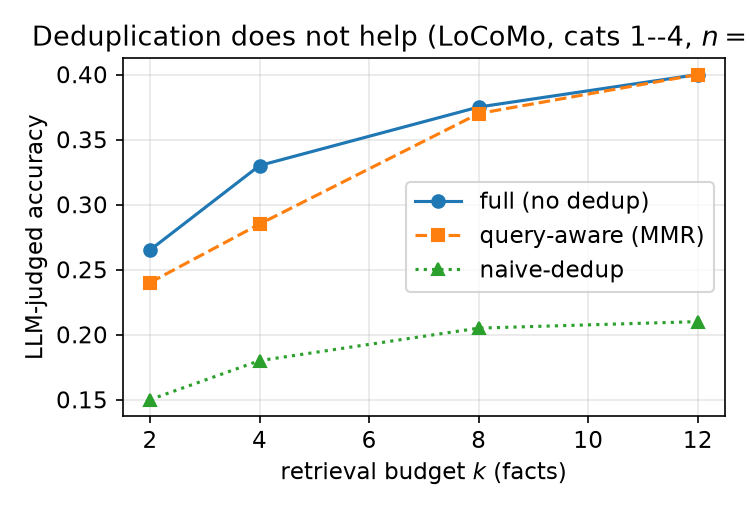
\includegraphics[width=\linewidth]{figures/fig_budget_sweep.png}
\caption{LLM-judged accuracy vs.\ retrieval budget. Naive deduplication is
dominated at every budget; redundancy-aware composition never exceeds plain
top-$k$.}
\label{fig:sweep}
\end{figure}

\begin{table}[t]
\centering
\small
\begin{tabular}{lcccc}
\toprule
policy & $k{=}2$ & $k{=}4$ & $k{=}8$ & $k{=}12$ \\
\midrule
full & 0.265 & 0.330 & 0.375 & 0.400 \\
naive-dedup & 0.150 & 0.180 & 0.205 & 0.210 \\
query-aware (MMR) & 0.240 & 0.285 & 0.370 & 0.400 \\
\bottomrule
\end{tabular}
\caption{LLM-judged accuracy vs.\ retrieval budget ($n{=}200$, categories 1--4).
Naive deduplication is dominated everywhere; redundancy-aware composition never
exceeds plain top-$k$.}
\label{tab:sweep}
\end{table}

\begin{table}[t]
\centering
\small
\begin{tabular}{lcc}
\toprule
policy & $k{=}8$ & $k{=}12$ \\
\midrule
full & 0.365 & 0.411 \\
naive-dedup & 0.152 & 0.163 \\
query-aware (MMR) & 0.358 & 0.433 \\
\midrule
\multicolumn{3}{l}{McNemar (query-aware vs.\ full):} \\
\multicolumn{3}{l}{\quad $k{=}8$: $b{=}31,c{=}33,\ p{=}0.90$ (n.s.)} \\
\multicolumn{3}{l}{\quad $k{=}12$: $b{=}29,c{=}23,\ p{=}0.49$ (n.s.)} \\
\bottomrule
\end{tabular}
\caption{Multi-hop (category 1), all $n{=}282$ questions. Redundancy-aware
composition is statistically indistinguishable from plain top-$k$; naive
deduplication remains dominated.}
\label{tab:multihop}
\end{table}

\paragraph{Takeaway.} On this pipeline, deduplication is not a useful lever:
blind merging harms accuracy, and redundancy-aware selection is safe but
inert. If accuracy is being lost, it is being lost elsewhere.

\section{The Bottleneck: Retrieval Precision, then Reasoning}
\label{sec:bottleneck}

To locate the lost accuracy we exploit LoCoMo's per-question \emph{gold
evidence} turn ids, which most work ignores. We compare, per question
($n{=}200$, LLM-judged):
\begin{itemize}
  \item \textbf{retrieved}: our top-$k$ pipeline ($k{=}12$);
  \item \textbf{oracle}: only the gold evidence turns (with session dates) in
  context---a perfect-retrieval ceiling;
  \item \textbf{full\_conv}: the entire multi-session conversation in context
  (no retrieval), with \texttt{num\_ctx}$=32768$ so nothing is truncated.
\end{itemize}

\paragraph{Retrieval precision leaves large headroom.}
Overall accuracy is $0.40$ (retrieved) vs.\ $0.61$ (oracle)---about $21$ points
lost to imperfect retrieval---and on multi-hop the gap is $0.41\!\to\!0.72$
(Table~\ref{tab:oracle}). This is real, measured headroom for a precision
retriever, consistent with recent conversational-memory retrieval
work~\cite{li2026evimem,ji2026mragent}.

\paragraph{Precision beats recall: more context distracts.}
Supplying the whole conversation is \emph{worse} than precise evidence on
multi-hop ($0.628$ vs.\ $0.721$), echoing distraction
effects~\cite{liu2023lost,cuconasu2024power}. The lever is retrieving the exact
evidence, not retrieving more.

\paragraph{Reasoning is a hard floor retrieval cannot cross.}
On temporal questions, even the oracle scores only $0.156$: the gold evidence
and session dates are present, but the model cannot perform the required date
arithmetic (e.g.\ ``yesterday'' relative to the session date). No retriever can
fix this---it is a reasoning/grounding limit, and it caps how much precision
retrieval alone can deliver.

\begin{figure}[t]
\centering
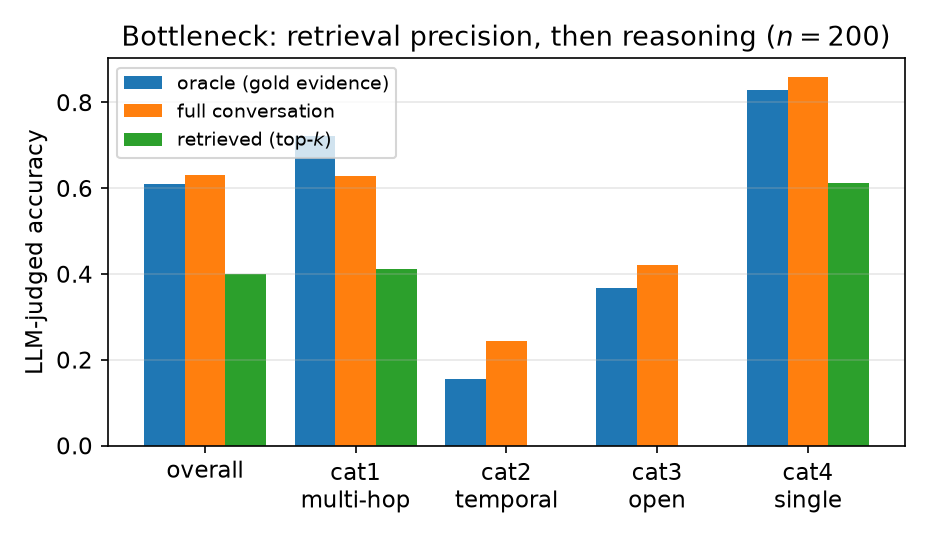
\includegraphics[width=\linewidth]{figures/fig_oracle.png}
\caption{Bottleneck decomposition ($n{=}200$). Oracle (gold evidence) far
exceeds retrieval, but temporal stays near-floor even with perfect evidence,
and full-context underperforms the oracle on multi-hop.}
\label{fig:oracle}
\end{figure}

\begin{table}[t]
\centering
\small
\begin{tabular}{lccccc}
\toprule
arm & overall & cat1 & cat2 & cat3 & cat4 \\
 & & (multi) & (temp) & (open) & (single) \\
\midrule
retrieved ($k{=}12$) & 0.400 & 0.411 & -- & -- & 0.613 \\
oracle & 0.610 & \textbf{0.721} & \textbf{0.156} & 0.368 & 0.828 \\
full\_conv & 0.630 & 0.628 & 0.244 & 0.421 & 0.860 \\
\bottomrule
\end{tabular}
\caption{Bottleneck decomposition ($n{=}200$, LLM-judged). Retrieval precision
leaves $\sim\!21$ points on the table; full-context \emph{distracts} on
multi-hop; temporal reasoning is near-floor \emph{even with gold evidence}.}
\label{tab:oracle}
\end{table}

\paragraph{Takeaway.} Effort ordering for small-model conversational memory:
deduplication (no effect) $<$ precision retrieval (bounded but real) $<$
reasoning/grounding (the ceiling). The temporal floor in particular is a
retrieval-invariant limit.

\section{Grounded Extractive Memory is Largely Faithful}
\label{sec:faithfulness}

A natural worry is that the LLM extractor writes \emph{hallucinated} facts into
memory that later corrupt answers---a concern formalized for open-ended
generation~\cite{min2023factscore,zhang2023snowball} and, for memory systems,
benchmarked by HaluMem~\cite{chen2025halumem}. We probe whether this is a strong
effect in our grounded setup.

For a sample of extracted facts we ask an LLM judge whether each fact is fully
supported by (stated or unambiguously entailed by) the source session it was
extracted from. In a $120$-fact sample, $0$ were judged unsupported
($\approx\!0\%$). The extractor over-\emph{produces} facts (it inflates the store
and creates the redundancy of \S\ref{sec:redundancy}) but does not
\emph{fabricate}: because it summarizes a provided transcript rather than
generating from parametric memory, it stays close to the source. This contrasts
with the $\sim\!42\%$ unsupported atomic facts reported for open-ended
biography generation~\cite{min2023factscore}.

\paragraph{Takeaway.} For grounded, extractive memory writes, hallucinated-memory
accumulation is a weak effect; the store's problem is \emph{quantity/redundancy}
and downstream \emph{retrieval/reasoning}, not fabrication. (This is a limited
probe---single extractor, single judge, one dataset, conservative
parse-handling---and is not a claim about generative or tool-use memory, where
HaluMem shows hallucination does accumulate.)

\section{Generality and Robustness}
\label{sec:generality}

Our main study fixes one small model and one dataset. We now probe whether the
two load-bearing findings---(i) deduplication does not help, and (ii) reasoning,
especially temporal, is a floor retrieval cannot cross---survive a change of
judge, a change of dataset, and a change of answerer.

\paragraph{A second, independent judge.} We re-judge the cached answers with a
different model, \texttt{llama3.2:3b} (vs.\ \texttt{qwen3:8b}). The two judges
agree on $81.3\%$ of $600$ items (Cohen's $\kappa = 0.52$, moderate);
\texttt{llama3.2} is stricter (positive rate $0.19$ vs.\ $0.31$). Crucially, the
\emph{policy ordering is identical} under the second judge: naive-dedup remains
dominated at every budget ($0.06$--$0.09$ vs.\ full $0.23$--$0.30$) and
query-aware $\approx$ full. Finding (i) is judge-robust; only the absolute scale
shifts.

\paragraph{A second dataset (LongMemEval).} We test finding (ii) on the
LongMemEval~\cite{wu2024longmemeval} oracle split, which supplies gold evidence
sessions per question, typed by reasoning kind. Answering from gold evidence
with \texttt{qwen3:8b} (Table~\ref{tab:lme}, Fig.~\ref{fig:lme}),
\emph{temporal-reasoning is the lowest type} ($0.275$), far below easy
single-session types ($0.80$--$0.95$), with multi-session (the multi-hop analog)
second-lowest ($0.375$). This mirrors LoCoMo, where temporal is also the worst
category with gold evidence ($0.156$). The temporal floor is not a LoCoMo
artifact: it replicates across two datasets and two question taxonomies.

\begin{table}[t]
\centering
\small
\begin{tabular}{lcc}
\toprule
question type & oracle acc. & $n$ \\
\midrule
single-session-assistant & 0.950 & 40 \\
single-session-user & 0.800 & 40 \\
knowledge-update & 0.600 & 40 \\
single-session-preference & 0.467 & 30 \\
multi-session & 0.375 & 40 \\
\textbf{temporal-reasoning} & \textbf{0.275} & 40 \\
\midrule
overall & 0.583 & 230 \\
\bottomrule
\end{tabular}
\caption{LongMemEval (oracle split), \texttt{qwen3:8b} answering from gold
evidence. Temporal reasoning is the floor even with perfect evidence,
replicating the LoCoMo result on a second dataset.}
\label{tab:lme}
\end{table}

\begin{figure}[t]
\centering
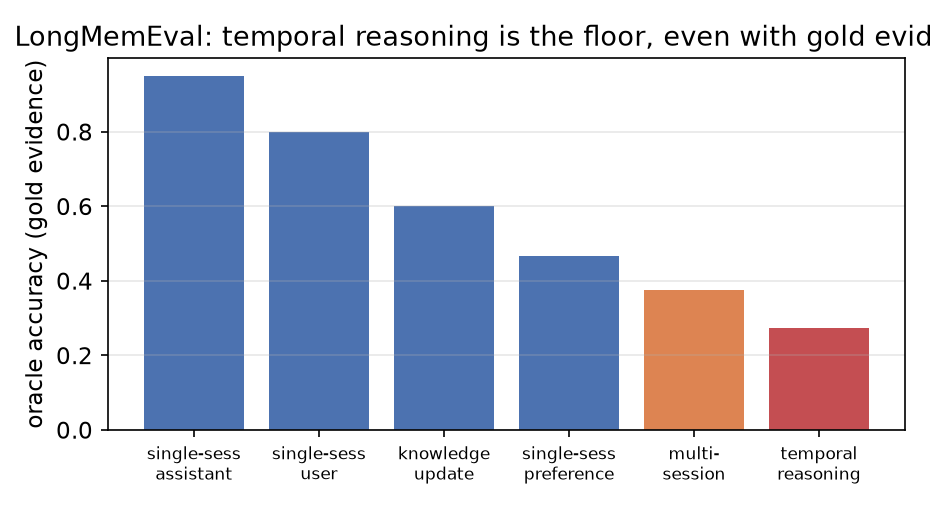
\includegraphics[width=\linewidth]{figures/fig_longmemeval.png}
\caption{LongMemEval oracle-answering accuracy by question type. Temporal
reasoning (right, red) is lowest despite gold evidence.}
\label{fig:lme}
\end{figure}

\paragraph{A second answerer model.} Finally we replace the answering model with
\texttt{llama3.2:3b} (retrieval and the qwen3-built store held fixed; judge held
fixed as \texttt{qwen3:8b}), at $k{=}8$ on $n{=}120$ questions per policy. The
ordering again replicates: naive-dedup is dominated ($0.192$ vs.\ full $0.342$)
and query-aware $\approx$ full ($0.333$). Finding (i) survives a change of the
generation model as well as the judge.

\paragraph{Summary.} The two load-bearing findings are robust to the axes we
could vary locally: deduplication fails to help under two judges and two
answerer models, and the temporal-reasoning floor appears under two datasets.
Absolute accuracies shift with model and judge; the qualitative conclusions do
not.

\section{Discussion}
\label{sec:discussion}

Our results give a consistent, if deflationary, picture for small-model
long-term conversational memory.

\paragraph{Redundancy is a red herring for accuracy.} It is real and large
(\S\ref{sec:redundancy}), and it is tempting to optimize---but neither removing
it (harmful) nor composing around it (inert) improves answers
(\S\ref{sec:dedup}). Deduplication may still matter for \emph{cost} (a similarity
gate halves the store), but not for quality in this regime. This complements,
rather than contradicts, redundancy-aware selection results on static-corpus
RAG~\cite{peng2025adagres}: the setting and objective differ.

\paragraph{Precision retrieval is the actionable lever, with a known cap.} The
$0.40\!\to\!0.61$ oracle gap (\S\ref{sec:bottleneck}) is exactly the headroom
that iterative, gap-driven conversational-memory
retrievers~\cite{li2026evimem,ji2026mragent} exploit. Our contribution here is to
\emph{quantify the cap}: full-context distraction and, decisively, a temporal
reasoning floor that no retriever crosses.

\paragraph{The temporal floor is the interesting residual.} That the oracle
scores $0.156$ on temporal questions---with gold evidence and dates in
context---isolates a reasoning/grounding failure (relative-to-absolute date
resolution) that is orthogonal to memory mechanisms. For small models this,
not redundancy or retrieval, is where accuracy is truly lost.

\paragraph{Why we report a diagnosis, not a method.} Each first-principles
mechanism we considered---semantic deduplication, precision multi-hop retrieval
over conversational memory, and hallucinated-memory mitigation---is already
covered by very recent work~\cite{peng2025adagres,li2026evimem,ji2026mragent,chen2025halumem}.
The subfield is moving quickly; the durable value we can add is a controlled,
reproducible decomposition that tells practitioners which lever to pull for a
small local stack.

\section{Limitations}
\label{sec:limitations}

This is a deliberately narrow, honest study and should be read as such.
\begin{itemize}
  \item \textbf{Scale of models and data.} The main study uses \texttt{qwen3:8b}
  with \texttt{nomic-embed}/\texttt{MiniLM} on LoCoMo. \S\ref{sec:generality}
  extends the two load-bearing findings to a second judge (\texttt{llama3.2:3b}),
  a second answerer (\texttt{llama3.2:3b}), and a second dataset
  (LongMemEval~\cite{wu2024longmemeval}), but all models are small and local;
  whether the conclusions hold for frontier models is untested. Absolute numbers
  are not competitive with frontier systems and are not meant to be---only the
  \emph{relative, within-pipeline} comparisons are claimed.
  \item \textbf{LLM-as-judge.} Scoring uses the same model family as generation;
  self-preference bias is possible. We mitigate by comparing arms under an
  identical judge, but a human-validated subset is future work.
  \item \textbf{Metric thresholds.} \mdr/\rtf{} are threshold- and
  embedder-dependent; we report curves rather than single numbers, and do not
  compare absolute \mdr{} across embedders.
  \item \textbf{Deduplication scope.} We test one blind-merge threshold and one
  redundancy-aware composer (MMR). A learned or store-level query-distribution
  method could differ, though our composition-level negative gives little reason
  to expect a large gain.
  \item \textbf{Faithfulness probe.} The $1/400$ result is a single-judge,
  single-extractor, conservative-parse probe; it bounds the effect as small in
  \emph{this} grounded setup, not in generative or tool-use memory.
  \item \textbf{No new method.} We claim a diagnosis, not a system that improves
  the state of the art.
\end{itemize}

\section{Conclusion}
\label{sec:conclusion}

We presented a controlled, fully reproducible anatomy of failure in a small,
local long-term conversational-memory pipeline. Redundancy in an LLM-built store
is real and semantic ($\sim\!62\%$ near-duplicates at $\tau{=}0.85$, invisible
to lexical matching), yet deduplication does not help: blind merging is
Pareto-dominated at every budget and redundancy-aware composition is
statistically indistinguishable from top-$k$ on multi-hop ($n{=}282$,
$p{=}0.90$). Using gold evidence as an oracle, we show the accuracy is lost to
retrieval precision ($0.40\!\to\!0.61$) and, decisively, to reasoning: temporal
questions remain near-floor ($0.156$) \emph{with perfect evidence}, and
full-context retrieval distracts. Grounded extractive memory is meanwhile
largely faithful. The practical message for small-model agent memory is an
effort ordering---deduplication is not the lever, precision retrieval helps but
is capped, and reasoning/grounding is the ceiling. Code, data, and all
experiment scripts are released at
\url{https://github.com/saisushaman/AI-MEMORY-}.


\bibliographystyle{plain}
\bibliography{references}

\end{document}
